\section{109 --- Convert Sorted List to Binary Search Tree}
Given a singly linked list where elements are sorted in ascending order, convert it to a height balanced BST.

For this problem, a height-balanced binary tree is defined as a binary tree in which the depth of the two subtrees of \textit{every} node never differ by more than 1.
\paragraph{Example:}
\begin{flushleft}
\textbf{Input}: \fcj{[-10,-3,0,5,9]},

One possible answer is: \fcj{[0,-3,9,-10,null,5]}, which represents the following height balanced \textbf{BST}:

\begin{figure}[H]
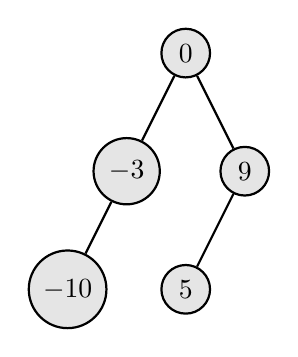
\begin{tikzpicture}
[every node/.style={draw, circle, fill=gray!20!, minimum size=5mm},
%level 1/.style={sibling distance=25mm},
%level 2/.style={sibling distance=15mm},
thick]
\node{0}
child{node{$-3$} child{node{$-10$}} child[missing]}
child{node{9} child{node{5}} child[missing]};
\end{tikzpicture}
\end{figure}

\end{flushleft}
\subsection{Recursion}
链表的查找中间点可以通过快慢指针来操。找到中点后,要以中点的值建立一个根节点,然后需要把原链表断开,分为前后两个链表,都不能包含原中点,

然后再分别对这两个链表递归调用原函数,分别连上左右子节点即可。
\setcounter{lstlisting}{0}
\begin{lstlisting}[style=customc, caption={Recursion}]
TreeNode* sortedListToBST( ListNode* head )
{
    if( head == nullptr )
    {
        return nullptr;
    }
    //find middle node
    ListNode* prev = nullptr;
    auto slow = head;
    auto fast = head;
    while( fast && fast->next )
    {
        prev = slow;
        slow = slow->next;
        fast = fast->next->next;
    }
    //break the linked list
    if( prev )
    {
        prev->next = nullptr;
    }
    //create tree node with the value of slow poiner
    auto node = new TreeNode( slow->val );
    //Base case when there is only one node in the linked list
    if( head == slow )
    {
        return node;
    }
    //left child tree is left half of slow
    node->left = sortedListToBST( head );
    //right child tree is right half of slow
    node->right = sortedListToBST( slow->next );
    return node;
}
\end{lstlisting}

\subsection{Inorder Simulation}
The critical idea based on the inorder traversal is:

\begin{itemize}
\item The leftmost element in the inorder traversal has to be the head of the given linked list.
\item Similarly, the next element in the inorder traversal will be the second element in the linked list and so on.
\end{itemize}

The above shows the relationship between the inorder traversal of a binary search tree and the linked list nodes.

\begin{enumerate}
\item Iterate over the linked list to find out it's length $L$. We will make use of two variables $S$ and $E$ to mark the beginning and the end of the list. They are set to 0 and $L - 1$ respectively.
\item We have to simulate the inorder traversal here. We can find out the middle element $M$ by using $(S + E) / 2$. Note that we don't really find out the middle node of the linked list. We just have a variable telling us the index of the middle element. We simply need this to make recursive calls on the two halves.
\item Recurse on the left half by using $S$, $M- 1$ as the starting and ending points.
\item The invariance maintained in this algorithm is that whenever the left half of the BST is completely built, the head pointer in the linked list will point to the root node or the middle node (which becomes the root). So, we simply use the current value pointed to by head as the root node and move the head to its next node.
\item We recurse on the right hand side using $M + 1$, $E$ as the starting and ending points.
\end{enumerate}

\begin{lstlisting}[style=customc, caption={Inorder Simulation}]
TreeNode* sortedListToBST( ListNode* head )
{
    auto node = head;
    //find the size of linked list
    int count = 0;
    while( node )
    {
        node = node->next;
        ++count;
    }
    //create binary search tree
    return create( 0, count - 1, head );
}
TreeNode* create( int l, int r, ListNode*& node )
{
    if( l > r )
    {
        return nullptr;
    }
    //find middle
    int mid = ( l + r ) / 2;
    //First step of simulated inorder traversal.
    auto left = create( l, mid - 1, node );
    //since node will be updated during the process
    //we put creating tree node after the above
    //traversel is completed
    auto t = new TreeNode( node->val );
    t->left = left;
    node = node->next;
    //recurse on the right hand side and form BST out of them
    t->right = create( mid + 1, r, node );
    return t;
}
\end{lstlisting}